61. \begin{figure}[ht!]
\center{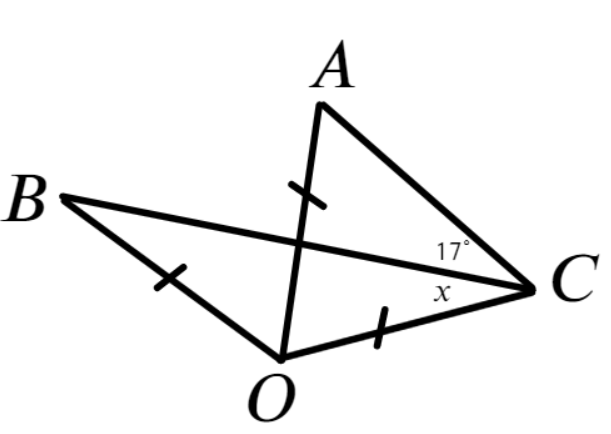
\includegraphics[scale=0.35]{g61.png}}
\end{figure}\\
Обозначим $\angle BCO=x.$ Треугольник $AOC$ равнобедренный с углом при основании $x+17^\circ,$ поэтому $\angle AOC=180^\circ-2\cdot(x+17^\circ)=146^\circ-2x.$ Треугольник $BOC$ равнобедренный с углом при основании $x,$ поэтому $\angle BOC=180^\circ-2x.$ Таким образом, $\angle AOB=180^\circ-2x-(146^\circ-2x)=34^\circ.$\\
